\documentclass[11pt]{article}
\newcommand{\tablelang}{uk}
% Shared preamble for docs/paper/tex/en/main.tex and docs/paper/tex/uk/main.tex (XeLaTeX via Tectonic).
% Same layout, fonts and packages as the author's earlier Zenodo preprint (10.5281/zenodo.23375871).
% The including file sets \mainlang{english} or \mainlang{ukrainian} before % Shared preamble for docs/paper/tex/en/main.tex and docs/paper/tex/uk/main.tex (XeLaTeX via Tectonic).
% Same layout, fonts and packages as the author's earlier Zenodo preprint (10.5281/zenodo.23375871).
% The including file sets \mainlang{english} or \mainlang{ukrainian} before % Shared preamble for docs/paper/tex/en/main.tex and docs/paper/tex/uk/main.tex (XeLaTeX via Tectonic).
% Same layout, fonts and packages as the author's earlier Zenodo preprint (10.5281/zenodo.23375871).
% The including file sets \mainlang{english} or \mainlang{ukrainian} before \input{../preamble}.
\usepackage[a4paper,margin=25mm]{geometry}
\usepackage{fontspec}
\setmainfont{cmunrm.otf}[BoldFont=cmunbx.otf,ItalicFont=cmunti.otf,BoldItalicFont=cmunbi.otf]
\setsansfont{cmunss.otf}[BoldFont=cmunsx.otf,ItalicFont=cmunsi.otf]
\setmonofont{cmuntt.otf}[BoldFont=cmuntb.otf,ItalicFont=cmunit.otf]
\usepackage[ukrainian,english]{babel}
\usepackage{amsmath,amssymb,amsthm,mathtools}
\usepackage{booktabs,tabularx,array,multirow}
\usepackage{graphicx}
\usepackage[font=small,labelfont=bf]{caption}
\usepackage{subcaption}
\usepackage{xcolor}
\usepackage{microtype}
\usepackage[numbers,sort&compress]{natbib}
\PassOptionsToPackage{hyphens}{url}
\usepackage[hidelinks]{hyperref}
\usepackage[nameinlink,capitalise,noabbrev]{cleveref}
\usepackage{url}
\usepackage{etoolbox}
\AtBeginEnvironment{thebibliography}{\raggedright}

\graphicspath{{../../figures/}}
% primitive input: LaTeX's \input is not expandable and breaks inside tabular after \midrule
\makeatletter\newcommand{\gentable}[1]{\@@input ../tables/\tablelang/T#1.tex }\makeatother

% theorem names: the including file may define these before \input{../preamble}
\providecommand{\lemmaname}{Lemma}
\providecommand{\propositionname}{Proposition}
\providecommand{\definitionname}{Definition}
\providecommand{\remarkname}{Remark}
\providecommand{\corollaryname}{Corollary}
\providecommand{\theoremname}{Theorem}
\theoremstyle{plain}
\newtheorem{lemma}{\lemmaname}
\newtheorem{proposition}{\propositionname}
\theoremstyle{definition}
\newtheorem{definition}{\definitionname}
\theoremstyle{remark}
\newtheorem{remark}{\remarkname}

\setlength{\tabcolsep}{4pt}
\renewcommand{\arraystretch}{1.12}
\newcommand{\code}[1]{\texttt{#1}}
\sloppy
.
\usepackage[a4paper,margin=25mm]{geometry}
\usepackage{fontspec}
\setmainfont{cmunrm.otf}[BoldFont=cmunbx.otf,ItalicFont=cmunti.otf,BoldItalicFont=cmunbi.otf]
\setsansfont{cmunss.otf}[BoldFont=cmunsx.otf,ItalicFont=cmunsi.otf]
\setmonofont{cmuntt.otf}[BoldFont=cmuntb.otf,ItalicFont=cmunit.otf]
\usepackage[ukrainian,english]{babel}
\usepackage{amsmath,amssymb,amsthm,mathtools}
\usepackage{booktabs,tabularx,array,multirow}
\usepackage{graphicx}
\usepackage[font=small,labelfont=bf]{caption}
\usepackage{subcaption}
\usepackage{xcolor}
\usepackage{microtype}
\usepackage[numbers,sort&compress]{natbib}
\PassOptionsToPackage{hyphens}{url}
\usepackage[hidelinks]{hyperref}
\usepackage[nameinlink,capitalise,noabbrev]{cleveref}
\usepackage{url}
\usepackage{etoolbox}
\AtBeginEnvironment{thebibliography}{\raggedright}

\graphicspath{{../../figures/}}
% primitive input: LaTeX's \input is not expandable and breaks inside tabular after \midrule
\makeatletter\newcommand{\gentable}[1]{\@@input ../tables/\tablelang/T#1.tex }\makeatother

% theorem names: the including file may define these before % Shared preamble for docs/paper/tex/en/main.tex and docs/paper/tex/uk/main.tex (XeLaTeX via Tectonic).
% Same layout, fonts and packages as the author's earlier Zenodo preprint (10.5281/zenodo.23375871).
% The including file sets \mainlang{english} or \mainlang{ukrainian} before \input{../preamble}.
\usepackage[a4paper,margin=25mm]{geometry}
\usepackage{fontspec}
\setmainfont{cmunrm.otf}[BoldFont=cmunbx.otf,ItalicFont=cmunti.otf,BoldItalicFont=cmunbi.otf]
\setsansfont{cmunss.otf}[BoldFont=cmunsx.otf,ItalicFont=cmunsi.otf]
\setmonofont{cmuntt.otf}[BoldFont=cmuntb.otf,ItalicFont=cmunit.otf]
\usepackage[ukrainian,english]{babel}
\usepackage{amsmath,amssymb,amsthm,mathtools}
\usepackage{booktabs,tabularx,array,multirow}
\usepackage{graphicx}
\usepackage[font=small,labelfont=bf]{caption}
\usepackage{subcaption}
\usepackage{xcolor}
\usepackage{microtype}
\usepackage[numbers,sort&compress]{natbib}
\PassOptionsToPackage{hyphens}{url}
\usepackage[hidelinks]{hyperref}
\usepackage[nameinlink,capitalise,noabbrev]{cleveref}
\usepackage{url}
\usepackage{etoolbox}
\AtBeginEnvironment{thebibliography}{\raggedright}

\graphicspath{{../../figures/}}
% primitive input: LaTeX's \input is not expandable and breaks inside tabular after \midrule
\makeatletter\newcommand{\gentable}[1]{\@@input ../tables/\tablelang/T#1.tex }\makeatother

% theorem names: the including file may define these before \input{../preamble}
\providecommand{\lemmaname}{Lemma}
\providecommand{\propositionname}{Proposition}
\providecommand{\definitionname}{Definition}
\providecommand{\remarkname}{Remark}
\providecommand{\corollaryname}{Corollary}
\providecommand{\theoremname}{Theorem}
\theoremstyle{plain}
\newtheorem{lemma}{\lemmaname}
\newtheorem{proposition}{\propositionname}
\theoremstyle{definition}
\newtheorem{definition}{\definitionname}
\theoremstyle{remark}
\newtheorem{remark}{\remarkname}

\setlength{\tabcolsep}{4pt}
\renewcommand{\arraystretch}{1.12}
\newcommand{\code}[1]{\texttt{#1}}
\sloppy

\providecommand{\lemmaname}{Lemma}
\providecommand{\propositionname}{Proposition}
\providecommand{\definitionname}{Definition}
\providecommand{\remarkname}{Remark}
\providecommand{\corollaryname}{Corollary}
\providecommand{\theoremname}{Theorem}
\theoremstyle{plain}
\newtheorem{lemma}{\lemmaname}
\newtheorem{proposition}{\propositionname}
\theoremstyle{definition}
\newtheorem{definition}{\definitionname}
\theoremstyle{remark}
\newtheorem{remark}{\remarkname}

\setlength{\tabcolsep}{4pt}
\renewcommand{\arraystretch}{1.12}
\newcommand{\code}[1]{\texttt{#1}}
\sloppy
.
\usepackage[a4paper,margin=25mm]{geometry}
\usepackage{fontspec}
\setmainfont{cmunrm.otf}[BoldFont=cmunbx.otf,ItalicFont=cmunti.otf,BoldItalicFont=cmunbi.otf]
\setsansfont{cmunss.otf}[BoldFont=cmunsx.otf,ItalicFont=cmunsi.otf]
\setmonofont{cmuntt.otf}[BoldFont=cmuntb.otf,ItalicFont=cmunit.otf]
\usepackage[ukrainian,english]{babel}
\usepackage{amsmath,amssymb,amsthm,mathtools}
\usepackage{booktabs,tabularx,array,multirow}
\usepackage{graphicx}
\usepackage[font=small,labelfont=bf]{caption}
\usepackage{subcaption}
\usepackage{xcolor}
\usepackage{microtype}
\usepackage[numbers,sort&compress]{natbib}
\PassOptionsToPackage{hyphens}{url}
\usepackage[hidelinks]{hyperref}
\usepackage[nameinlink,capitalise,noabbrev]{cleveref}
\usepackage{url}
\usepackage{etoolbox}
\AtBeginEnvironment{thebibliography}{\raggedright}

\graphicspath{{../../figures/}}
% primitive input: LaTeX's \input is not expandable and breaks inside tabular after \midrule
\makeatletter\newcommand{\gentable}[1]{\@@input ../tables/\tablelang/T#1.tex }\makeatother

% theorem names: the including file may define these before % Shared preamble for docs/paper/tex/en/main.tex and docs/paper/tex/uk/main.tex (XeLaTeX via Tectonic).
% Same layout, fonts and packages as the author's earlier Zenodo preprint (10.5281/zenodo.23375871).
% The including file sets \mainlang{english} or \mainlang{ukrainian} before % Shared preamble for docs/paper/tex/en/main.tex and docs/paper/tex/uk/main.tex (XeLaTeX via Tectonic).
% Same layout, fonts and packages as the author's earlier Zenodo preprint (10.5281/zenodo.23375871).
% The including file sets \mainlang{english} or \mainlang{ukrainian} before \input{../preamble}.
\usepackage[a4paper,margin=25mm]{geometry}
\usepackage{fontspec}
\setmainfont{cmunrm.otf}[BoldFont=cmunbx.otf,ItalicFont=cmunti.otf,BoldItalicFont=cmunbi.otf]
\setsansfont{cmunss.otf}[BoldFont=cmunsx.otf,ItalicFont=cmunsi.otf]
\setmonofont{cmuntt.otf}[BoldFont=cmuntb.otf,ItalicFont=cmunit.otf]
\usepackage[ukrainian,english]{babel}
\usepackage{amsmath,amssymb,amsthm,mathtools}
\usepackage{booktabs,tabularx,array,multirow}
\usepackage{graphicx}
\usepackage[font=small,labelfont=bf]{caption}
\usepackage{subcaption}
\usepackage{xcolor}
\usepackage{microtype}
\usepackage[numbers,sort&compress]{natbib}
\PassOptionsToPackage{hyphens}{url}
\usepackage[hidelinks]{hyperref}
\usepackage[nameinlink,capitalise,noabbrev]{cleveref}
\usepackage{url}
\usepackage{etoolbox}
\AtBeginEnvironment{thebibliography}{\raggedright}

\graphicspath{{../../figures/}}
% primitive input: LaTeX's \input is not expandable and breaks inside tabular after \midrule
\makeatletter\newcommand{\gentable}[1]{\@@input ../tables/\tablelang/T#1.tex }\makeatother

% theorem names: the including file may define these before \input{../preamble}
\providecommand{\lemmaname}{Lemma}
\providecommand{\propositionname}{Proposition}
\providecommand{\definitionname}{Definition}
\providecommand{\remarkname}{Remark}
\providecommand{\corollaryname}{Corollary}
\providecommand{\theoremname}{Theorem}
\theoremstyle{plain}
\newtheorem{lemma}{\lemmaname}
\newtheorem{proposition}{\propositionname}
\theoremstyle{definition}
\newtheorem{definition}{\definitionname}
\theoremstyle{remark}
\newtheorem{remark}{\remarkname}

\setlength{\tabcolsep}{4pt}
\renewcommand{\arraystretch}{1.12}
\newcommand{\code}[1]{\texttt{#1}}
\sloppy
.
\usepackage[a4paper,margin=25mm]{geometry}
\usepackage{fontspec}
\setmainfont{cmunrm.otf}[BoldFont=cmunbx.otf,ItalicFont=cmunti.otf,BoldItalicFont=cmunbi.otf]
\setsansfont{cmunss.otf}[BoldFont=cmunsx.otf,ItalicFont=cmunsi.otf]
\setmonofont{cmuntt.otf}[BoldFont=cmuntb.otf,ItalicFont=cmunit.otf]
\usepackage[ukrainian,english]{babel}
\usepackage{amsmath,amssymb,amsthm,mathtools}
\usepackage{booktabs,tabularx,array,multirow}
\usepackage{graphicx}
\usepackage[font=small,labelfont=bf]{caption}
\usepackage{subcaption}
\usepackage{xcolor}
\usepackage{microtype}
\usepackage[numbers,sort&compress]{natbib}
\PassOptionsToPackage{hyphens}{url}
\usepackage[hidelinks]{hyperref}
\usepackage[nameinlink,capitalise,noabbrev]{cleveref}
\usepackage{url}
\usepackage{etoolbox}
\AtBeginEnvironment{thebibliography}{\raggedright}

\graphicspath{{../../figures/}}
% primitive input: LaTeX's \input is not expandable and breaks inside tabular after \midrule
\makeatletter\newcommand{\gentable}[1]{\@@input ../tables/\tablelang/T#1.tex }\makeatother

% theorem names: the including file may define these before % Shared preamble for docs/paper/tex/en/main.tex and docs/paper/tex/uk/main.tex (XeLaTeX via Tectonic).
% Same layout, fonts and packages as the author's earlier Zenodo preprint (10.5281/zenodo.23375871).
% The including file sets \mainlang{english} or \mainlang{ukrainian} before \input{../preamble}.
\usepackage[a4paper,margin=25mm]{geometry}
\usepackage{fontspec}
\setmainfont{cmunrm.otf}[BoldFont=cmunbx.otf,ItalicFont=cmunti.otf,BoldItalicFont=cmunbi.otf]
\setsansfont{cmunss.otf}[BoldFont=cmunsx.otf,ItalicFont=cmunsi.otf]
\setmonofont{cmuntt.otf}[BoldFont=cmuntb.otf,ItalicFont=cmunit.otf]
\usepackage[ukrainian,english]{babel}
\usepackage{amsmath,amssymb,amsthm,mathtools}
\usepackage{booktabs,tabularx,array,multirow}
\usepackage{graphicx}
\usepackage[font=small,labelfont=bf]{caption}
\usepackage{subcaption}
\usepackage{xcolor}
\usepackage{microtype}
\usepackage[numbers,sort&compress]{natbib}
\PassOptionsToPackage{hyphens}{url}
\usepackage[hidelinks]{hyperref}
\usepackage[nameinlink,capitalise,noabbrev]{cleveref}
\usepackage{url}
\usepackage{etoolbox}
\AtBeginEnvironment{thebibliography}{\raggedright}

\graphicspath{{../../figures/}}
% primitive input: LaTeX's \input is not expandable and breaks inside tabular after \midrule
\makeatletter\newcommand{\gentable}[1]{\@@input ../tables/\tablelang/T#1.tex }\makeatother

% theorem names: the including file may define these before \input{../preamble}
\providecommand{\lemmaname}{Lemma}
\providecommand{\propositionname}{Proposition}
\providecommand{\definitionname}{Definition}
\providecommand{\remarkname}{Remark}
\providecommand{\corollaryname}{Corollary}
\providecommand{\theoremname}{Theorem}
\theoremstyle{plain}
\newtheorem{lemma}{\lemmaname}
\newtheorem{proposition}{\propositionname}
\theoremstyle{definition}
\newtheorem{definition}{\definitionname}
\theoremstyle{remark}
\newtheorem{remark}{\remarkname}

\setlength{\tabcolsep}{4pt}
\renewcommand{\arraystretch}{1.12}
\newcommand{\code}[1]{\texttt{#1}}
\sloppy

\providecommand{\lemmaname}{Lemma}
\providecommand{\propositionname}{Proposition}
\providecommand{\definitionname}{Definition}
\providecommand{\remarkname}{Remark}
\providecommand{\corollaryname}{Corollary}
\providecommand{\theoremname}{Theorem}
\theoremstyle{plain}
\newtheorem{lemma}{\lemmaname}
\newtheorem{proposition}{\propositionname}
\theoremstyle{definition}
\newtheorem{definition}{\definitionname}
\theoremstyle{remark}
\newtheorem{remark}{\remarkname}

\setlength{\tabcolsep}{4pt}
\renewcommand{\arraystretch}{1.12}
\newcommand{\code}[1]{\texttt{#1}}
\sloppy

\providecommand{\lemmaname}{Lemma}
\providecommand{\propositionname}{Proposition}
\providecommand{\definitionname}{Definition}
\providecommand{\remarkname}{Remark}
\providecommand{\corollaryname}{Corollary}
\providecommand{\theoremname}{Theorem}
\theoremstyle{plain}
\newtheorem{lemma}{\lemmaname}
\newtheorem{proposition}{\propositionname}
\theoremstyle{definition}
\newtheorem{definition}{\definitionname}
\theoremstyle{remark}
\newtheorem{remark}{\remarkname}

\setlength{\tabcolsep}{4pt}
\renewcommand{\arraystretch}{1.12}
\newcommand{\code}[1]{\texttt{#1}}
\sloppy


% ---- additions local to the Ukrainian article (preamble.tex left unchanged) ----
\newcolumntype{L}{>{\raggedright\arraybackslash}X}
\newcolumntype{R}{>{\raggedleft\arraybackslash}X}
\newcolumntype{P}[1]{>{\raggedright\arraybackslash}p{#1}}
\newcommand{\en}[1]{\foreignlanguage{english}{#1}}
% Ukrainian cleveref names (cleveref has no Ukrainian support)
\crefname{section}{розділ}{розділи}
\Crefname{section}{Розділ}{Розділи}
\crefname{subsection}{підрозділ}{підрозділи}
\Crefname{subsection}{Підрозділ}{Підрозділи}
\crefname{appendix}{додаток}{додатки}
\Crefname{appendix}{Додаток}{Додатки}
\crefname{table}{таблиця}{таблиці}
\Crefname{table}{Таблиця}{Таблиці}
\crefname{figure}{рисунок}{рисунки}
\Crefname{figure}{Рисунок}{Рисунки}
\setlength{\emergencystretch}{2em}
\hypersetup{pdftitle={Більше, ніж пройдені тести: огляд специфікації лише за інтерфейсом скорочує тихі збої локального агента-програміста на Gemma},
  pdfauthor={Олександр Пилипенко},
  pdfkeywords={агенти-програмісти, великі мовні моделі, тестування за специфікацією, тихі збої, Gemma, Gemini, Google Antigravity, попередня реєстрація}}

\begin{document}
\selectlanguage{ukrainian}

\title{Більше, ніж пройдені тести: огляд специфікації лише за інтерфейсом скорочує тихі збої локального агента-програміста на Gemma}
\author{Олександр Пилипенко\\[2pt]\small Незалежний дослідник у сфері штучного інтелекту та машинного навчання\\ \small Аспірант Державного торговельно-економічного університету, Київ, Україна\\ \small У співпраці з кафедрою інженерії програмного забезпечення та кібербезпеки\\[2pt]
\small ORCID: \href{https://orcid.org/0009-0004-9610-9242}{0009-0004-9610-9242}\\ \small\href{mailto:O.Pylypenko@knute.edu.ua}{\texttt{O.Pylypenko@knute.edu.ua}}}
\date{2026-10-21}
\maketitle

\begin{abstract}
\noindent
Агенти-програмісти зазвичай зупиняються після проходження доступних тестів, навіть якщо ті не охоплюють сформульованих вимог. Ми досліджуємо цей збій у схемі «хмарний архітектор / локальний виконавець», де \code{gemma4:12b} виправляє невеликі модулі Python на ноутбучному GPU. Хмарний рецензент отримує лише сигнатури, docstring і поля типів даних, ніколи тіла функцій, та повертає контрактні тести або чекліст. Окрема прихована перевірка оцінює отриманий код. На 50 екземплярах задач і 150 парних запусках із виправленим вимірюванням група контрактних тестів зменшила тихі хибні успіхи з 37 до 4 і підвищила верифіковане виконання з 66{,}0\% до 87{,}3\%; на рівні задач тихі збої зменшилися у 12 випадках і не зросли в жодному ($p=0{,}0005$, post hoc). Це об'єднані задачі, частково використані під час розробки, а не 50 незалежних нових специфікацій. У зареєстрованій кампанії на 25 нових задачах обидві форми огляду підвищили верифіковане виконання з 58/75 до 71/75 і зменшили тихі хибні успіхи з 9/75 до 1/75. Чекліст дав ту саму сукупну частку верифікованого виконання, що й контрактні тести; еквівалентність не перевірялася. З урахуванням одноразової генерації на задачу, повторно використаної для трьох seed, час кампанії зріс на 11{,}8\% для чекліста і на 53{,}7\% для тестів. Зареєстрований тест на рівні задач не досяг значущості ($p=0{,}125$); приріст контрактних тестів зосереджений у багатофайлових задачах. Розвідувальна абляція вказує на важливість docstring. Результати підтримують застосування огляду специфікації в цих обмежених умовах; його причинні складові та ефективність на дефектах реальних репозиторіїв залишаються відкритими питаннями.
\end{abstract}

\noindent\textbf{Ключові слова:} агенти-програмісти; великі мовні моделі; тестування за специфікацією; тестові оракули; тихі збої; Gemma; Gemini; Google Antigravity; попередня реєстрація.

\medskip
\noindent\textbf{Незалежність від Google.} Дослідження оцінює архітектурну схему, яку Google описав публічно; воно не узгоджувалося з Google, не спонсорувалося і не рецензувалося ним, і жодних тверджень про продукти Google, окрім процитованого оголошення, не робиться. Усі експерименти виконано на обладнанні та облікових записах автора.

% =====================================================================
\section{Вступ}\label{sec:intro}
Пройдений набір тестів --- звичайний критерій зупинки для автономного агента-програміста. Водночас він слабкий: коли тести покривають лише частину специфікації, агент може задовольнити тести й порушити решту. Дослідження бенчмарків показали, що недостатні тести завищують коректність згенерованого коду: розширення тестів HumanEval знизило pass@$k$ на 19{,}3--28{,}9\% для 26 моделей~\citep{liu2023evalplus}. Для агента, що працює без нагляду, така помилка гірша за видиму: агент повідомляє про успіх, і ніщо далі не заперечує.

Ми натрапили на цей збій, будуючи гібридний оркестратор, у якому хмарний «архітектор» планує, а локальна модель редагує код, щоб вихідний код залишався на машині. Саме таку схему Google запропонував для локальних моделей в Antigravity SDK: хмарна модель Gemini планує лише за назвами файлів і описами, а локальні екземпляри Gemma виконують роботу на пристрої~\citep{kotwani2026antigravity}. З локальним виконавцем на 12B параметрів головним збоєм на задачах із насиченою специфікацією була не нездатність редагувати код чи йти за планом: виконавець проходив видимі тести й мовчки пропускав правила, сформульовані лише в docstring. Збільшення ліміту генерації, режим міркування при повторній спробі, підказки хмари після невдалої спроби та одноетапна адаптація обв'язки цього не змінили (\cref{sec:res-negative}).

Ця стаття ставить вузьке питання: \textbf{чи може хмарна модель, що читає лише специфікацію і пише контрактні тести або чекліст правил, зменшити тихі збої локального агента-програміста так, щоб реалізація не залишала машину, і якою ціною?} Наші внески:
\begin{enumerate}
\item Вимірювання тихих хибних успіхів локального агента-програміста на задачах із насиченою специфікацією з незалежною прихованою перевіркою як еталоном.
\item Механізм з обмеженим розкриттям, у якому хмара бачить лише сигнатури, docstring і поля типів даних, і докази того, що повнота інтерфейсу визначає, допомагають контрактні тести чи шкодять.
\item Попередньо зареєстрована кампанія з контрольним чеклістом, що перевіряє, чи додає виконуваність огляду вимірювану користь, і процедура побудови задач (жеребкування видимих правил; баги локальної моделі), що зменшує свободу автора обирати умови на користь методу.
\item Оцінювання, що розділяє висновки на рівні запусків і на рівні задач, звітує негативні результати для п'яти альтернативних втручань і перевіряє згенеровані тести на надмірну суворість і мутаційне покриття без участі агента.
\end{enumerate}
Ми не стверджуємо, що генерація тестів мовними моделями є новою (\cref{sec:related}), ані що ефект поширюється за межі досліджуваного класу задач (\cref{sec:limitations}).

% =====================================================================
\section{Пов'язані роботи}\label{sec:related}
\paragraph{Недостатні тести.} EvalPlus розширив вхідні дані тестів HumanEval приблизно у 80 разів за допомогою генерації мовними моделями та мутацій і виявив, що багато розв'язків, раніше визнаних правильними, хибні~\citep{liu2023evalplus}. Наші приховані перевірки відіграють роль сильніших тестів; нас цікавить власний критерій зупинки агента, а не оцінювання бенчмарка.

\paragraph{Тести, згенеровані мовними моделями.} CodeT генерує тести тією самою моделлю, що пише кандидатні розв'язки, і впорядковує розв'язки за узгодженістю з цими тестами~\citep{chen2023codet}. AgentCoder відокремлює агента-програміста від агента-тестувальника, який пише тести за вимогами~\citep{huang2024agentcoder}. TestGen-LLM у Meta покращує наявні тестові класи, написані людьми, і залишає лише кандидатів, що проходять фільтри вимірюваного покращення; у впровадженні 75\% тестів скомпілювалися, 57\% надійно проходили, а 25\% підвищили покриття~\citep{alshahwan2024testgen}. Найближча до нашої постановки робота --- генерація тестів за специфікацією в Google: спершу виводяться передумови, післяумови й невизначена поведінка, а потім за ними пишуться тести; це підвищило виявлення помилок на виробничих багах на 9{,}8 відсоткового пункту ($p=0{,}0352$)~\citep{tufano2026contracts}. Наш механізм відрізняється напрямком потоку інформації: тести пише \emph{інша, віддалена} модель, яка ніколи не бачить тіл функцій, а тести слугують критерієм приймання для \emph{локального} агента, а не продуктом-набором тестів.

\paragraph{Агенти, що обходять тести.} ImpossibleBench змінює тести так, що вони суперечать специфікації природною мовою, і вимірює, як часто агенти все одно їх проходять~\citep{zhong2026impossiblebench}. Наш тип збою доповнювальний: агент не маніпулює тестами; він зупиняється, щойно видимі тести пройдено, і лишає нереалізованими правила, яких тести не перевіряють.

\paragraph{Адаптація обв'язки.} Harness$^2$ адаптує обв'язку агента --- промпти, процедури, інструменти --- без зміни ваг моделі~\citep{harness2}. Одноетапна адаптація нашого виконавця в цьому стилі не покращила результат на відкладених задачах (\cref{sec:res-negative}).

\paragraph{Тестові оракули, самозворотний зв’язок і зовнішня валідність.} Проблема оракула полягає у визначенні очікуваної поведінки навіть за автоматичної генерації входів; специфікації й контракти є усталеними джерелами оракулів~\citep{barr2015oracle}. Наші приховані тести --- операційний оракул, а не повна специфікація. Self-Refine повідомляє про покращення завдяки ітеративному самозворотному зв’язку~\citep{madaan2023selfrefine}, а Huang та співавтори виявляють обмеження внутрішньої самокорекції міркувань без зовнішнього зворотного зв’язку~\citep{huang2024selfcorrect}; різні умови застерігають від узагальнення нашого негативного результату SPEC. SWE-bench досліджує реальні дефекти репозиторіїв~\citep{jimenez2024swebench}, а LiveCodeBench збирає нові задачі для зменшення ризику контамінації~\citep{jain2024livecodebench}. Тут ми не оцінюємо жоден із цих бенчмарків. Приховані правила контролюють доступ до оцінювання в експерименті, але не доводять відсутності контамінації навчання чи перенесення на реальні дефекти.

% =====================================================================
\section{Постановка задачі та метрики}\label{sec:problem}
Задача складається з модуля з дефектом, функції якого мають специфікації в docstring, файлу видимих модульних тестів і прихованої перевірки, яка перевіряє правила docstring, пропущені видимими тестами. Для одного запуску агента нехай $V\in\{0,1\}$ означає, що власні видимі тести задачі проходять після запуску, $H\in\{0,1\}$ --- що проходить прихована перевірка, а $S\in\{0,1\}$ --- що агент повідомляє про успіх.
\begin{itemize}
\item \textbf{Верифіковане виконання} (основна метрика): $V=1\land H=1$.
\item \textbf{Тихий хибний успіх:} $S=1\land(V=0\lor H=0)$; на практиці майже завжди $V=1$, $H=0$.
\item \textbf{Вартість:} час запуску агента, локальні й хмарні токени, а також одноразова генерація огляду для задачі.
\end{itemize}
$V$ і $H$ оцінює бенчмарк після запуску лише на власних тестових модулях задачі (згенеровані контрактні тести виключено); прихована перевірка ніколи не показується жодній із моделей.

Тут \emph{верифіковане виконання} означає успіх за визначеною процедурою оцінювання, а не доведення повної функціональної коректності. Прихована перевірка сама пропускає деякі правила docstring (\cref{sec:res-quality}).

% =====================================================================
\section{Система}\label{sec:system}
\paragraph{Локальний агент.} \code{gemma4:12b} в Ollama 0.33.3 (дайджест моделі \code{4eb23ef187e2\ldots}) з власним викликом інструментів над набором інструментів робочої теки (читання, запис і латання файлів; запуск команди перевірки), без режиму міркування, з контекстом 16\,384 токени, лімітом генерації 2\,048 токенів, який для однієї повторної спроби підвищується до 4\,096, коли виклик інструмента обрізано, підказками етапу, що називають наступний крок і тест, який не проходить, та циклом самовиправлення до двох спроб із дедлайном 300\,с на спробу. Обладнання: один ноутбучний GPU NVIDIA GeForce RTX 4060 (8\,ГБ) і 31\,ГБ RAM; модель частково вивантажується на CPU.

\paragraph{Інтерфейсне навантаження.} Для файлів, які може змінювати підзадача, і нетестових вхідних модулів, якими вони користуються, обхід AST видає назви класів, сигнатури функцій, docstring і анотовані поля класів (назви й типи; значення за замовчуванням відкинуто). Тіла функцій та решту коду пропущено, а навантаження перед виходом із машини проходить перевірник приватності оркестратора.

\paragraph{Автор контрактних тестів.} Хмарна модель отримує навантаження та інструкцію написати один модуль \code{unittest}, що перевіряє кожне правило docstring --- результати для типових і граничних входів та \code{ValueError} для кожного описаного виду некоректного входу --- і не перевіряти нічого, чого docstring не стверджує. Отриманий модуль статично перевіряється (імпорти лише \code{unittest} і модулів, що тестуються; без \code{open}, \code{exec}, \code{eval}, \code{getattr} тощо; без dunder-атрибутів; наявний підклас \code{TestCase}) і, якщо коректний, записується поруч із власними тестами задачі як \code{test\_spec\_contract.py}, де його знаходить звичайна команда перевірки агента. Тести генеруються один раз для задачі й повторно використовуються для всіх seed. Хмарний бекенд --- Antigravity CLI (\code{agy} 1.4.3), запущений у порожній тимчасовій теці з інструкцією не використовувати інструменти. У прогонах R1--R5 використовувалася модель CLI за замовчуванням, яку не було зафіксовано; у кампаніях A і B модель задано явно.

\paragraph{Автор чекліста.} Для контрольної групи та сама хмарна модель отримує те саме навантаження й повертає пронумерований перелік правил docstring без коду; перелік додається до опису задачі, який читає агент.

\paragraph{Межа приватності.} Назви, типи й docstring самі можуть розкривати інформацію; тому ми описуємо механізм як \emph{обмежене розкриття специфікації}, а не як формальну гарантію приватності.

\begin{figure}[tb]
\centering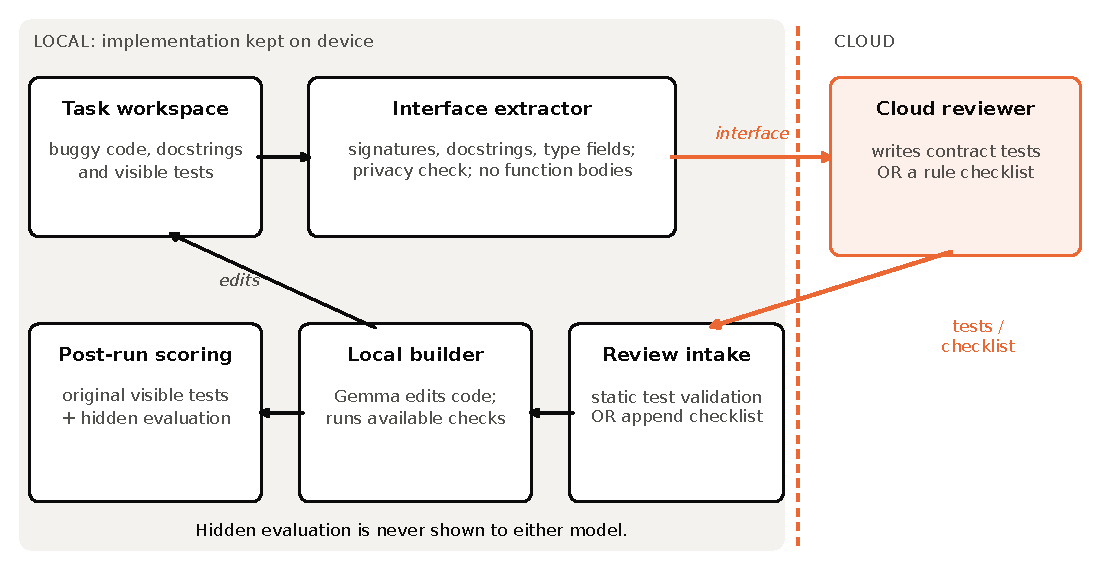
\includegraphics[width=\linewidth]{fig1_architecture.pdf}
\caption{Потік інформації. Межу з хмарою перетинає лише інтерфейс (сигнатури, docstring, поля типів), а назад повертається лише статично перевірений модуль модульних тестів (або чекліст правил); агент редагує код локально, доки не пройде видимі й контрактні тести. Рішення про приймання ухвалюється після запуску за власними видимими тестами задачі та прихованою перевіркою, якої не бачить жодна модель.}\label{fig:architecture}
\end{figure}

% =====================================================================
\section{Дизайн експериментів}\label{sec:design}
Усі запуски в усіх групах використовують однаковий цикл агента, дедлайн і ліміт спроб, по три seed (303, 404, 505) на задачу, з чергуванням порядку груп для кожного seed. Задачі --- невеликі задачі з виправлення коду на Python (один-два модулі), у яких видимі тести покривають лише частину docstring; кожну задачу перевірено заздалегідь: початковий код і часткові виправлення не проходять, а еталонні виправлення проходять і видимі, і приховані перевірки.

Докази зібрано у п'яти прогонах на 19 задачах (\cref{tab:runs}) та у двох зареєстрованих кампаніях: A на 25 нових специфікаціях і B на шести повторно використаних. Прогони R1--R3 були розвідувальними; між R3 і R4 знайдено й виправлено помилку вимірювання (\cref{sec:res-measurement}); R4 було попередньо зареєстровано; R5 повторює порівняння R3 з виправленим вимірюванням.

\begin{table}[tb]
\centering\small
\caption{Прогони на перших 19 задачах.}\label{tab:runs}
\begin{tabularx}{\linewidth}{@{}llLLL@{}}
\toprule
Прогін & Коміт & Задачі & Групи & Мета \\
\midrule
R1 & \code{cc938ca} & H6, H9--H13 (6) & базова, SPEC, SPECTESTS, ASSIST & розвідувальне порівняння \\
R2 & \code{24fbe35} & H1--H5, H7, H8 (7) & базова, SPECTESTS v1 & шкода на розв'язаних задачах \\
R3 & \code{750647e} & H1--H13 (13) & базова, SPECTESTS v2 & порівняння в одній сесії \\
R4 & \code{7a369ac} & H14--H19 (6, нові) & базова, SPECTESTS v2 & зареєстроване підтвердження \\
R5 & \code{7a369ac}/\code{2c59e38} & H1--H13 (13) & базова, SPECTESTS v2 & повтор із виправленим вимірюванням \\
\bottomrule
\end{tabularx}
\end{table}

\emph{Базова політика} --- агент із підказками етапу й адаптивним лімітом генерації. \emph{SPEC} після проходження видимих тестів дає агентові сигнатури й docstring його задачі та вимагає одноразової самоперевірки кожного правила. \emph{SPECTESTS} встановлює хмарні контрактні тести до запуску (v1: лише власний файл функцій; v2: також поля типів даних і залежні модулі). \emph{ASSIST} після невдалої спроби просить у хмари покрокові вказівки. Між R3 і R4 для обох груп внесено зміну: одиничне застрягання в межах спроби тепер дає нову спробу, а не завершує підзадачу.

\paragraph{Попередня реєстрація R4.} До будь-якого запуску на H14--H19 основну кінцеву точку (верифіковане виконання), групи, seed, ліміт спроб, парування за (задача, seed) і точний двосторонній знаковий тест було записано в журнал прогонів проєкту. Журнал --- локальний файл поза системою контролю версій, тому ця реєстрація не має незалежної часової мітки (\cref{sec:limitations}). Перша спроба R4 упала на зависанні й використала невиправлене вимірювання; її відкинуто й повторено без змін, окрім виправлення вимірювання.

\paragraph{Статистика.} Порівняння на рівні запусків використовують точні двосторонні знакові тести на розбіжних парах (задача, seed). Оскільки запуски однієї задачі не є незалежними, ми також аналізуємо різницю частки верифікованого виконання для кожної задачі (контрактні тести мінус базова політика, за трьома seed): знаковий тест на рівні задач, точний перестановочний тест зі зміною знаків і кластерний бутстреп за задачами (20\,000 повторень). Аналіз на рівні задач додано після зовнішньої рецензії; щодо R4 він є post hoc.

\paragraph{Підтверджувальні кампанії A і B.} Щоб відповісти на загрози з \cref{sec:limitations} --- задачі й баги, написані автором уже після виявлення типу збою, замало нових задач, незафіксована хмарна модель і відсутність контролю на те, що хмара просто читає специфікацію, --- ще дві кампанії було зареєстровано публічними комітами до їх запуску (\cref{app:prereg}).
\begin{itemize}
\item \emph{Задачі.} Двадцять п'ять нових задач із виправлення коду (P1--P25: 8 однофайлових, 10 багатофайлових, 7 зі свідомо стислими, недовизначеними docstring) з предметних областей, яких раніше не було (гроші, текст, дати, одиниці, розклад, статистика, конфігурація, матриці, обмеження частоти, форматування). Кожен docstring формулює пронумеровані правила, і кожне правило має тестові випадки. \textbf{Які правила покривають видимі тести, автор не обирає:} для кожного правила вирішує жереб із фіксованим seed ($p=0{,}5$) з єдиним обмеженням: щонайменше одне видиме правило має не проходити на коді з дефектом. Прихована перевірка перевіряє всі правила. Вміст задач заморожено за SHA-256 для кожної задачі.
\item \emph{Баги.} У кампанії A код із дефектом пише автор. У кампанії B його пише сама локальна модель: для кожної специфікації \code{gemma4:12b} реалізує модуль за скелетом із docstring (seed генерації 1--5, температура 0{,}8, тести не показуються); оригінальні docstring відновлюються, щоб дефект був лише в тілах функцій, а першою задачею стає перша реалізація, яка порушує правило. Специфікації, які модель реалізує правильно на всіх seed, виключаються й підраховуються.
\item \emph{Групи.} Базова політика; контрактні тести; та \textbf{контрольна група «чекліст»}. Контроль порівнює форми огляду за тієї самої хмарної моделі й інтерфейсу; він не ізолює потужність моделі чи незалежність. Кампанія A додає розвідувальну абляцію того, скільки інтерфейсу бачить хмара (лише сигнатури; плюс docstring; повний).
\item \emph{Налаштування.} Як у R4--R5, із зафіксованою хмарною моделлю (Gemini 4 Argon у кампанії A; Gemini 3.8 Flash у кампанії B за зареєстрованою поправкою) та окремим записом часу одноразової генерації для кожної задачі. Seed 303, 404, 505. Основний тест: точний двосторонній знаковий тест за задачами для частки верифікованого виконання (контрактні тести проти базової); вторинні: тихі хибні успіхи, контрактні тести проти чекліста, результати за категоріями, вартість.
\end{itemize}

% =====================================================================
\section{Результати}\label{sec:results}

\subsection{Розвідувальне порівняння (R1)}\label{sec:res-r1}
На шести задачах із насиченою специфікацією верифіковане виконання становило 7/18 для базової політики, 5/18 з локальною самоперевіркою (SPEC), 16/18 з контрактними тестами (SPECTESTS) і 8/18 з підказками після невдачі (ASSIST); SPECTESTS проти базової дали 10 перемог і 1 поразку ($p=0{,}012$ на рівні запусків). Запусків, що пройшли видимі тести, але не пройшли прихованої перевірки, було 11 для базової, 10 для SPEC, 0 для SPECTESTS і 10 для ASSIST. R1 оцінював групу SPECTESTS за суворішим критерієм, ніж базову (\cref{sec:res-measurement}).

\subsection{Повнота інтерфейсу вирішує між допомогою і шкодою (R2, R3)}\label{sec:res-interface}
На семи задачах, які базова політика вже розв'язує, перша версія контрактних тестів (v1), написана лише за власним файлом функцій, знизила верифіковане виконання з 21/21 до 15/21 (0 перемог, 6 поразок, $p=0{,}031$). П'ять поразок припало на H1 і H3, де типи даних визначено в інших модулях; перевірка згенерованих модулів на еталонних реалізаціях показала 19 з 20 хибних тестів для H1 (неіснуюча назва поля) і 11 з 12 для H3 (пропущений аргумент конструктора). Коли в навантаження додано поля типів і залежні модулі (v2), кожен згенерований модуль для 13 задач пройшов на своїй еталонній реалізації, а розв'язані задачі втратили 2 з 21 запуску (незначущо); на чотирьох задачах, де базова здебільшого зупинялася на видимих тестах, верифіковане виконання зросло з 2/12 до 10/12 (8 перемог, 0 поразок, $p=0{,}0078$).

\subsection{Зареєстрований прогін на нових задачах (R4)}\label{sec:res-r4}
На шести раніше не використаних задачах верифіковане виконання становило 4/18 для базової і 11/18 з контрактними тестами (8 перемог, 1 поразка, 9 нічиїх; $p=0{,}039$ на рівні запусків), а тихих хибних успіхів було 14/18 і 3/18. На рівні задач покращилися три задачі (H14 0/3$\to$3/3, H15 0/3$\to$3/3, H16 0/3$\to$1/3), погіршень не було, три не змінилися: знаковий тест $p=0{,}25$, середній приріст $+0{,}39$ (95\% CI кластерного бутстрепу 0{,}06--0{,}72). Усі три тихі збої, що залишилися, припали на H17; єдині порушені приховані правила стосуються порожніх пар (\code{"a=1;;b=2"}, \code{"a=1;"}), а таке прочитання docstring спірне; оцінка H17 без цих двох випадків дала 7/18 проти 14/18 з тими самими 8 перемогами й 1 поразкою. Усі шість згенерованих модулів пройшли на незалежних еталонних реалізаціях.

\subsection{Усі 19 задач із виправленим вимірюванням (R4 + R5)}\label{sec:res-19}
R5 повторив порівняння R3 на H1--H13 з виправленим вимірюванням: 28/39 проти 37/39 (10 перемог, 1 поразка, $p=0{,}012$ на рівні запусків), тихі хибні успіхи 11/39 проти 0/39, а на дев'яти задачах, які базова розв'язує 3/3, верифіковано 26 з 27 запусків SPECTESTS (одна поразка на H6). Разом для R4 і R5 (19 задач, однаковий рушій і перевірки) верифіковане виконання становило 32/57 проти 48/57, а тихі хибні успіхи 25/57 проти 3/57. \Cref{tab:tasklevel} і \cref{fig:pertask} показують картину на рівні задач, а \cref{fig:silent} --- тихі хибні успіхи. Приріст зосереджено в семи задачах, правила яких сформульовано лише в docstring (H9, H10, H12, H13, H14, H15, H16); одинадцять задач не змінилися, а одна (H6) втратила один запуск із трьох.

\begin{table}[tb]
\centering\small
\caption{Аналіз R4 і R5 на рівні задач (одиниця --- задача; різниця частки верифікованого виконання за трьома seed, контрактні тести мінус базова політика).}\label{tab:tasklevel}
\begin{tabularx}{\linewidth}{@{}LcccL@{}}
\toprule
Набір & Краще/гірше/рівно & Знаковий тест $p$ & Зміна знаків $p$ & Середній приріст (95\% CI бутстрепу) \\
\midrule
\gentable{2}
\bottomrule
\end{tabularx}
\end{table}

\begin{figure}[tb]
\centering
\begin{subfigure}[t]{0.52\linewidth}\centering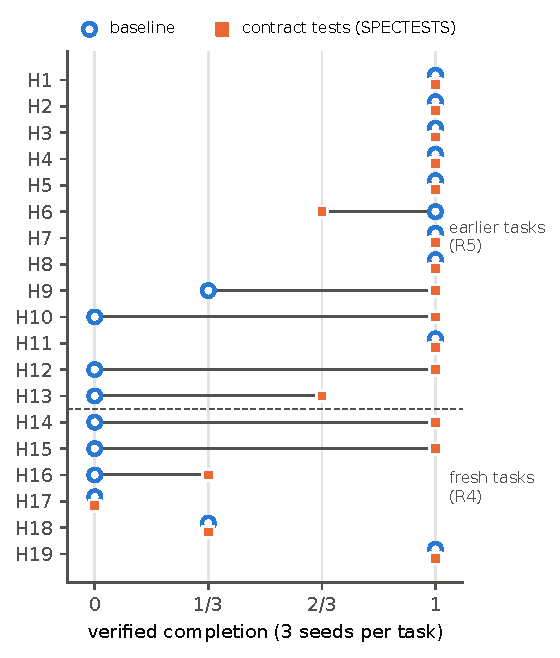
\includegraphics[width=\linewidth]{fig2_per_task.pdf}\caption{Верифіковане виконання за задачами.}\label{fig:pertask}\end{subfigure}\hfill
\begin{subfigure}[t]{0.46\linewidth}\centering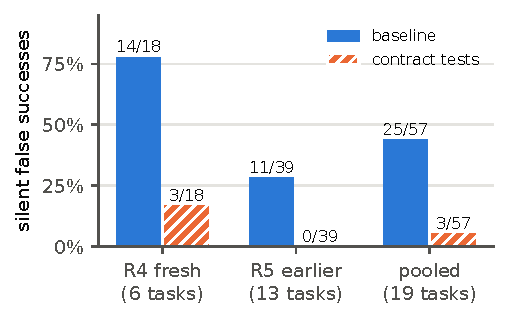
\includegraphics[width=\linewidth]{fig3_silent.pdf}\caption{Тихі хибні успіхи.}\label{fig:silent}\end{subfigure}
\caption{R4 і R5. (a) Верифіковане виконання для кожної задачі (три seed) для базової політики (порожні кола) і з контрактними тестами (заповнені квадрати); задачі нижче пунктирної лінії --- нові задачі зареєстрованого прогону R4. (b) Запуски, у яких агент повідомив про успіх, а незалежна перевірка не пройшла.}\label{fig:r45}
\end{figure}

\subsection{Якість згенерованих тестів}\label{sec:res-quality}
Згенеровані тести досліджено без участі агента. \textbf{Надмірна суворість.} Сорок сім різних реалізацій, які в запусках \emph{без} контрактних тестів пройшли і видимі тести, і приховану перевірку, відтворено із записаних diff (геші початкового стану звірено) і прогнано на контрактних модулях v2: не пройшли 6 із 91 пари «реалізація--модуль», усі на H4 (від'ємна вага має викликати помилку) і H9 (знак \code{+} або не-ASCII символ у prerelease має бути відхилено). У кожному випадку docstring формулює правило, а реалізація його порушує; прихована перевірка цього правила не перевіряє. Жодного контрактного тесту, що вимагав би поведінки, якої docstring не формулює, не знайдено. \textbf{Мутаційне покриття.} Із 448 одноточкових AST-мутантів еталонних реалізацій (19 задач) прихована перевірка вбила 333; із них видимі тести вбили 205 (61{,}6\%), а контрактні модулі v2 --- усіх (469 з 469 оцінених пар «мутант--модуль»; один мутант може оцінюватися кількома модулями, тому цей знаменник відрізняється від 333 унікальних мутантів; \cref{fig:mutation}). Ще 84 мутанти пережили приховану перевірку, але були вбиті контрактними тестами; кожен із них під час перегляду порушує правило docstring. Тридцять один мутант пережив усі перевірки. Для H14--H16 еталоном слугувала реалізація з прогону з контрактними тестами, що пройшла приховану перевірку, бо жоден запуск базової політики цих задач не розв'язав. Наслідок: приховані перевірки слабші за специфікації, тож «верифіковано» завищує коректність в обох групах; оскільки контрактні тести забезпечують пропущені правила, це упередження грає на користь базової політики.

\begin{figure}[tb]
\centering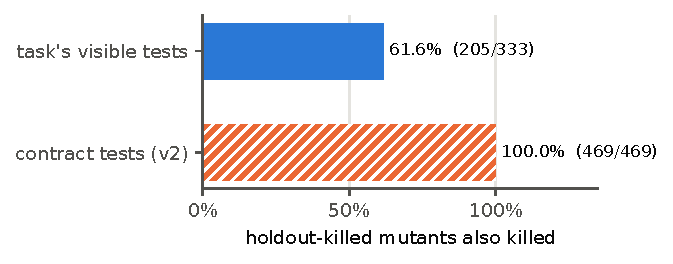
\includegraphics[width=0.78\linewidth]{fig4_mutation.pdf}
\caption{Із одноточкових мутантів, яких убиває прихована перевірка, частка, яку також убивають видимі тести задачі та контрактні тести v2 (для контрактних тестів --- пари «мутант--модуль»).}\label{fig:mutation}
\end{figure}

\subsection{Виправлення вимірювання і вартість}\label{sec:res-measurement}
У R1--R3 незалежна видима перевірка для групи SPECTESTS запускала також згенеровані тести, а прихована перевірка виконувалася лише за умови, що ця перевірка пройшла; тому запуски SPECTESTS оцінювалися суворіше, ніж запуски базової політики, що могло лише знизити їхні оцінки. R4, R5 і обидві кампанії використовують виправлені перевірки (лише власні тести задачі, прихована перевірка завжди виконується, зависання вважається невдачею).

Контрактні тести подовжують запуски: у R4 сумарний час становив 929\,с проти 4\,014\,с, а локальні токени --- 256\,017 проти 1\,171\,194, плюс 91\,958 хмарних токенів на шість викликів генерації; у R5 --- 3\,092\,с проти 5\,273\,с і 614\,904 проти 1\,378\,211 локальних токенів, плюс приблизно 264\,000 хмарних токенів на 13 задач. Базова політика швидка почасти тому, що зупиняється, щойно пройдено слабкі видимі тести. Ці значення часу не включають одноразову хмарну генерацію для задачі, яку в R1--R5 не вимірювали; співвідношення (1{,}7--4{,}3$\times$) є нижніми оцінками повної вартості. Кампанії записують час генерації окремо.

\subsection{Втручання, що не допомогли}\label{sec:res-negative}
\begin{itemize}
\item \textbf{Самоперевірка тією самою моделлю} (SPEC, R1): 5/18 проти 7/18; самоперевірки агента перевіряли лише ту поведінку, яку він уже реалізував.
\item \textbf{Підказки хмари після невдачі} (ASSIST, R1): 8/18; підказка вмикається після невдалої спроби, а перша спроба зазвичай проходила видимі тести, тож вона спрацювала один раз на 18 запусків.
\item \textbf{Ескалація ліміту генерації, міркування при повторі та допомога хмари} у двоспробовій драбині: на H6--H8 відмінності дала одна задача, і їх віднесено до розкиду між запусками.
\item \textbf{Одноетапна адаптація обв'язки} у стилі Harness$^2$~\citep{harness2}: на відкладених задачах обв'язка за замовчуванням верифікувала 7/12 запусків, а адаптовані --- 6/12, із довшим сумарним часом (829\,с проти 601\,с); стандартне правило відбору та правило з перевіркою зробили однакові вибори на кожній задачі, тож експеримент їх не розрізняє.
\end{itemize}

\subsection{Кампанія A: 25 нових задач із жеребкуванням видимих правил (зареєстрована)}\label{sec:res-a}
Виконано всі 225 основних запусків (3 групи $\times$ 25 задач $\times$ 3 seed). Для кожної задачі та форми огляду один етап генерації (до двох спроб) використовував Gemini 4 Argon; отримані артефакти повторно використано для всіх seed. Валідні модулі тестів установлено для 24 задач; надано 25 чеклістів (\cref{tab:campaign-a}, \cref{fig:campaign-a}).

\begin{table}[tb]
\centering\small
\caption{Кампанія A, усі запуски (25 задач $\times$ 3 seed). Генерація --- одноразовий виклик хмари для задачі.}\label{tab:campaign-a}
\begin{tabularx}{\linewidth}{@{}Lrrrrr@{}}
\toprule
Група & Верифіковано & Тихі хибні успіхи & Час запусків & Генерація & Хмарні токени \\
\midrule
\gentable{3}
\bottomrule
\end{tabularx}
\end{table}

\begin{figure}[tb]
\centering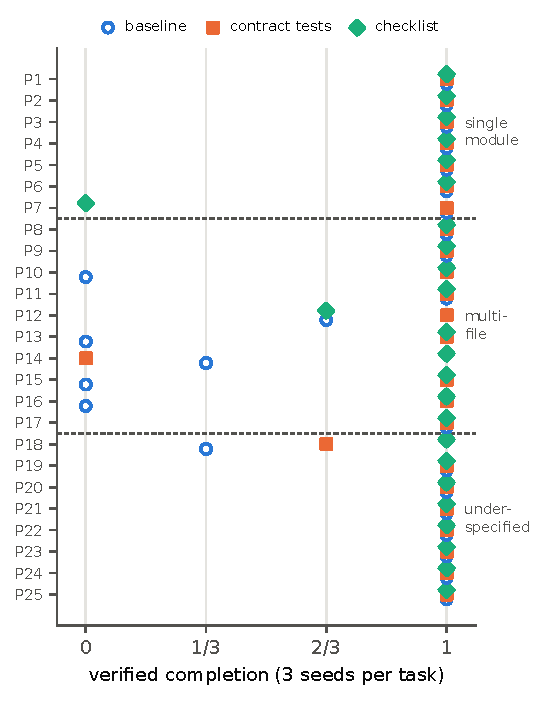
\includegraphics[width=0.55\linewidth]{fig5_campaign_a.pdf}
\caption{Кампанія A: верифіковане виконання для кожної задачі (три seed) для базової політики (порожні кола), контрактних тестів (квадрати) і контрольного чекліста (ромби). Пунктирні лінії розділяють однофайлові, багатофайлові й недовизначені задачі.}\label{fig:campaign-a}
\end{figure}

\paragraph{Основну гіпотезу (H1) не підтверджено.} На рівні задач контрактні тести покращили 6 задач і погіршили 1 (18 без змін): знаковий тест $p=0{,}125$, перестановочний тест $p=0{,}0625$, середній приріст частки верифікованого виконання $+0{,}17$ (95\% CI кластерного бутстрепу 0{,}04--0{,}33). Напрям збігається з попередніми прогонами, але зареєстрований тест не досягає $\alpha=0{,}05$. Тихих хибних успіхів (H2) стало менше в 3 задачах і більше в жодній ($p=0{,}25$).

Додатний бутстреп-інтервал для середнього й незначущий знаковий тест не суперечать одне одному. Знаковий тест використовує лише напрям ненульових ефектів задач, а бутстреп оцінює їхню середню величину за емпіричною вибіркою. Основним правилом рішення залишається зареєстрований знаковий тест; інтервал його не замінює.

\paragraph{Переваги над чеклістом не виявлено (H3).} Чекліст дав ту саму сукупну частку верифікованого виконання, що й контрактні тести (71/75), і ту саму кількість тихих хибних успіхів (1/75). На окремих задачах результати різнилися: тести проти чекліста --- 2 краще, 2 гірше, 21 рівно ($p=1{,}0$). Межу еквівалентності або не меншої ефективності не реєстрували й не перевіряли; незначуща різниця не доводить жодного з цих тверджень. Виконуваність не була необхідною для отримання цих сукупних результатів, але порівняння не ізолює причину користі огляду.

\paragraph{Де ефект.} Для контрактних тестів проти базової політики всі зміни припали на 10 багатофайлових задач (6 краще, 1 гірше; середнє $+0{,}43$). Базова політика вже проходила кожен запуск 8 однофайлових і 7 недовизначених задач. Через цей ефект стелі первинний знаковий тест має лише сім розбіжних задач. Чекліст окремо погіршив однофайлову CSV-задачу P7 (нижче). Контрактні тести не погіршили жодної задачі без прихованих порушень.

\paragraph{Невдачі двох хмарних груп.} P14 з контрактними тестами не вдалася 3/3: агент вичерпав спроби, а (правильні) контрактні тести так і не пройшли; P7 з чеклістом не вдалася 3/3 так само, після того як чекліст розписав правила лапок у CSV; обидва випадки --- явні невдачі. Для P18 обидва згенеровані модулі тестів відхилив статичний перевірник (вони використовували \code{\_\_dict\_\_}), тож група з контрактними тестами на цій задачі працювала без тестів, як і передбачала реєстрація.

\paragraph{Надійність генерації.} Валідний модуль установлено на 24/25 задачах (96\%); одна задача (P18, 4\%) залишилася без модуля після відхилення обох дозволених спроб генерації. Це частота на рівні задач, а не окремих відповідей. Три запуски P18 збережено в аналізі за призначеною групою (intention-to-treat). Збій хмарного бекенду зупиняє прогін; статичне відхилення є результатом роботи методу.

\paragraph{Якість згенерованих тестів.} На еталонних виправленнях не пройшли 4 тести в 3 з 24 встановлених модулів: три надмірно суворі --- на недовизначеній P20 вони вимагають \code{ValueError} для порожнього списку й дробового результату, а на P12 тест вимагає, щоб делегування до \code{statcore.mean} було видно для підміни (monkey-patching), що залежить від способу імпорту, а не від поведінки; четвертий (P10) очікує дробове \code{0.0} там, де docstring каже 0.0, а еталон повертає ціле 0. Жоден із цих тестів не спричинив невдалого запуску.

\paragraph{Скільки інтерфейсу потрібно хмарі (розвідувальна абляція, seed 303).} Лише із сигнатурами контрактні тести залишили верифіковане виконання на рівні базової політики (19/25, 2 тихі; базова 20/25 на цьому seed); додавання docstring дало 25/25 (0 тихих); повний інтерфейс із полями типів дав 23/25 (1 тихий). На цих задачах цінність міститься в docstring; поля типів тут нічого не додали, тоді як на H1 і H3, типи даних яких визначено в окремих модулях, їх відсутність породила неможливі тести (\cref{sec:res-interface}). Один seed на рівень, тож різниця в один-два запуски перебуває в межах розкиду.

\paragraph{Вартість з урахуванням генерації.} Сума часу запусків і одноразової генерації на задачу становила 6\,674{,}85\,с для базової політики, 10\,255{,}96\,с для контрактних тестів і 7\,459{,}95\,с для чекліста: накладні витрати кампанії 53{,}7\% і 11{,}8\% відповідно. Сам час запусків зріс на 44{,}3\% і 4{,}6\%. Кожен згенерований артефакт повторно використано для трьох seed, тож це амортизована вартість кампанії, а не виміряні витрати одноразового застосування. Вона не включає налаштування програм, аналіз і людську працю та не вимірює енергію чи гроші. У R1--R5 генерацію не вимірювали; їхні часові співвідношення не є повними витратами.

\subsection{Кампанія B: баги, написані локальною моделлю (зареєстрована; описова)}\label{sec:res-b}
\paragraph{Побудова.} Коли \code{gemma4:12b} попросили реалізувати кожну з 25 специфікацій кампанії A за скелетом із docstring, вона написала правильний модуль на всіх п'яти seed генерації для 19 специфікацій (104 генерації; одну відхилено як неповну). Природний баг дали лише шість специфікацій (N1, N7, N8, N9, N13, N18), що менше за зареєстрований поріг у десять, тож кампанію B звітовано описово, як і зареєстровано. У чотирьох із шести жереб зробив усі порушені правила видимими; лише N7 і N18 мають правила, порушені в прихованій формі. За пронумерованих правил у docstring локальна модель рідко лишає сформульоване правило нереалізованим, коли пише код з нуля; тихі збої попередніх задач виникали, коли вона виправляла код за неповними тестами.

\paragraph{Результати.} Виконано всі 54 запуски з Gemini 3.8 Flash як хмарною моделлю (\cref{tab:campaign-b}). На N18 контрактні тести верифікувалися в 3 з 3 запусків, чекліст --- в 1 з 3, базова --- в жодному; на N13 допоміг лише чекліст (2 з 3); N7, згенерований парсер якої зациклюється на деяких входах, не розв'язала жодна група. Усі шість згенерованих модулів тестів пройшли на еталонних виправленнях. На шести задачах ці результати описові; вони вказують у тому самому напрямку, що й кампанія A, причому контрактні тести --- єдина група без жодного тихого хибного успіху.

\begin{table}[tb]
\centering\small
\caption{Кампанія B, усі запуски (6 задач $\times$ 3 seed; описово).}\label{tab:campaign-b}
\begin{tabularx}{\linewidth}{@{}Lrrrrr@{}}
\toprule
Група & Верифіковано & Тихі хибні успіхи & Час запусків & Генерація & Хмарні токени \\
\midrule
\gentable{5}
\bottomrule
\end{tabularx}
\end{table}

\subsection{Об'єднані докази (post hoc)}\label{sec:res-pooled}
Об'єднання всіх запусків із виправленим вимірюванням --- R4, R5 і кампаній A та B, 50 задач, контрактні тести проти базової політики на тій самій задачі й seed --- дає загальний розмір ефекту (\cref{tab:pooled}). Цей аналіз визначено після прогонів і подано як описову підтримку, а не як зареєстрований тест. На рівні запусків у кампанії A контрактні тести виправили 15 запусків, у яких базова зазнала невдачі, і зламали 2 ($p=0{,}002$), а чекліст виправив 17 і зламав 4 ($p=0{,}007$); обидва усунули 9 з 10 розбіжних тихих хибних успіхів ($p=0{,}02$). Запуски з різними seed однієї задачі не незалежні, тож значення на рівні запусків завищують силу доказів для нових задач; значення на рівні задач є консервативнішим підсумком.

\paragraph{Чутливість до спільних специфікацій (post hoc).} 50 екземплярів охоплюють 19 попередніх задач, 25 задач кампанії A і 6 варіантів специфікацій A у кампанії B. Об’єднання кожної Pk з її варіантом Nk дає 44 групи за походженням специфікації. Усередині групи об’єднуємо запуски; у знаковому тесті кожна група має однакову вагу: верифіковане виконання покращується у 13 групах і погіршується у 2 ($p=0{,}00739$); тихі хибні успіхи зменшуються у 12 і не зростають у жодній ($p=0{,}000488$). Ця перевірка не встановлює незалежності всіх груп, а враховує одну відому залежність. Об’єднаний аналіз залишається розвідувальним. Скрипт: \code{scripts/analysis/publication.py}.

\begin{table}[tb]
\centering\small
\caption{Об'єднані запуски з виправленим вимірюванням (50 задач $\times$ 3 seed; post hoc).}\label{tab:pooled}
\begin{tabularx}{\linewidth}{@{}Lrrr@{}}
\toprule
Показник & Базова & Контрактні тести & Задач краще/гірше (знаковий тест $p$) \\
\midrule
\gentable{4}
\bottomrule
\end{tabularx}
\end{table}

% =====================================================================
\section{Обговорення}\label{sec:discussion}
\paragraph{Прогалина в покритті критерію зупинки.} Спостережувані збої узгоджуються з недостатнім покриттям критерію зупинки: агент часто зупинявся після проходження видимих тестів і залишав нереалізовані правила docstring. Альтернативні втручання не показали надійного приросту за перевірених задач і бюджетів (\cref{sec:res-negative}); це не свідчить про їхню неефективність в інших умовах.

\paragraph{Що встановлює контроль.} Чекліст і виконувані тести дали однакові сукупні результати кампанії A, а виміряний час кампанії був меншим для чекліста (11{,}8\% проти 53{,}7\% накладних витрат із генерацією). Це узгоджується з користю явного подання вимог специфікації. Дослідження не розділяє внески незалежності рецензента, потужності моделі, структурованого подання, додаткової явної інформації й моменту її надання. Зокрема, SPEC був локальною самоперевіркою після проходження видимих тестів, а не локальним чеклістом, створеним до виправлення. Його невдача не доводить необхідності незалежності й потужності моделі окремо. Майбутнє зареєстроване порівняння має зафіксувати момент і інтерфейс та порівняти локальний чекліст до виправлення, хмарний чекліст і безпосереднє подання початкових правил. Тести залишаються виконуваними артефактами аудиту, але додаткової переваги виконання над чеклістом тут не виявлено; еквівалентність не встановлено.

\paragraph{Розкриття та надмірна суворість.} Абляція на одному seed вказує, що docstring містили корисну інформацію понад сигнатури. Поля типів були необхідні для деяких попередніх задач, але в кампанії A не дали виміряного приросту. Неповні, неоднозначні або залежні від реалізації вимоги можуть породжувати надмірно суворі тести, зокрема на P12 поза категорією недовизначених задач. Жоден спостережуваний невдалий запуск не приписано розглянутим надмірним вимогам; це не доводить їхньої безпечності в інших умовах.

\paragraph{Межі й наступна перевірка.} Приріст контрактних тестів у кампанії A зосереджений у багатофайлових задачах; простіші задачі часто мали стельовий baseline. Це мотивує майбутню політику вибіркового огляду, але автоматичний вибір і межу вартості застосування тут не оцінювали. Сильніша зовнішня перевірка має зафіксувати новий набір реальних дефектів репозиторіїв із незалежними еталонними виправленнями й тестами та звітувати його окремо від сконструйованих тут задач.

\paragraph{Сила доказів.} Ефект має однаковий напрям у кожному експерименті, а в об'єднанні всіх виправлених запусків він великий: тихих хибних успіхів стало менше в 12 задачах і більше в жодній, а невдач --- менше в 14 і більше у 2 (\cref{tab:pooled}). Зареєстрований тест на рівні задач лише для кампанії A не досяг значущості (6 краще, 1 гірше, $p=0{,}125$), бо базова політика вже розв'язала 15 з 25 задач і розбіжних задач було лише сім. Тому головним результатом ми подаємо розмір і послідовність ефекту, а зареєстрований тест --- як межу того, наскільки його підтверджено на нових задачах.

% =====================================================================
\section{Обмеження та загрози валідності}\label{sec:limitations}
\begin{itemize}
\item \textbf{Добір задач.} Усі задачі --- невеликі задачі з виправлення коду на Python, написані автором. Перші 19 задач частково написано \emph{після} виявлення типу збою, і вони надмірно представляють задачі, де метод допомагає. Кампанія A зменшує це упередження (які правила видимі, вирішує жереб), а кампанія B бере баги від локальної моделі, але самі специфікації все ще авторські, з явно сформульованими й пронумерованими правилами, що робить їх легшими за типові docstring реального коду. Розмір ефекту на природних багах невідомий.
\item \textbf{Повторне використання під час розробки.} Задачі H1--H13 використовувалися під час розробки механізму; R4 і кампанія A використовують нові задачі; кампанія B має нові згенеровані реалізації з помилками для шести специфікацій A, а не нові специфікації.
\item \textbf{Одиниця аналізу і потужність.} Seed однієї задачі не є незалежними; $p$-значення на рівні запусків завищують узагальнення на нові задачі. Тести на рівні задач для R4--R5 (\cref{tab:tasklevel}) є post hoc; у кампанії A зареєстрований тест на рівні задач не був значущим переважно тому, що базова політика вже розв'язала більшість задач.

\item \textbf{Причинний висновок і спільні специфікації.} Генерація огляду одночасно змінює модель, подання, інформацію й момент її надання. SPEC не є узгодженим контролем із чеклістом до виправлення. Шість задач кампанії B повторно використовують специфікації A, тому 50 екземплярів не є 50 незалежними специфікаціями; аналіз чутливості на 44 групах є post hoc.
\item \textbf{Попередня реєстрація.} Реєстрація R4 зберігається в локальному журналі поза контролем версій і не має незалежної часової мітки; кампанії A і B зареєстровано публічними комітами до запуску, з однією задокументованою поправкою до кампанії B (хмарна модель).
\item \textbf{Еталон.} Приховані перевірки слабші за docstring (\cref{sec:res-quality}); частки верифікованого виконання є верхніми оцінками для обох груп.
\item \textbf{Межі: одна пара моделей.} Це дослідження однієї конфігурації: Gemma як локальний виконавець і хмарна модель за Antigravity CLI як рецензент. Оголошення Google поєднує Gemma 4 26B A4B з Gemini 3.8 Flash~\citep{kotwani2026antigravity}; ми використовуємо меншу \code{gemma4:12b}, Gemini 4 Argon у кампанії A і Gemini 3.8 Flash у кампанії B. У R1--R5 використовувалася модель CLI за замовчуванням, яку не зафіксовано, тож для цих прогонів не стверджується, що це була Gemini. Щодо інших сімейств моделей жодних тверджень не робиться, а порівняння між кампаніями A і B є описовими.
\item \textbf{Обладнання.} Один споживчий GPU з частковим вивантаженням на CPU; час виконання чутливий до фонового навантаження.
\item \textbf{Облік вартості.} У R1--R5 бракує часу хмарної генерації.
\item \textbf{Перервані прогони.} R5 і кампанії A та B призупинялися на прохання автора й відновлювалися із збережених результатів з тими самими згенерованими тестами й чеклістами, у різних сесіях.
\end{itemize}

% =====================================================================
\section{Доступність даних і коду}\label{sec:availability}
Код і артефакти доступні в \url{https://github.com/cyberdid/antigravity-codex-orchestrator}, гілка \code{main}. Зафіксований знімок експериментальних даних --- коміт \code{9cd894f717a4235c7cb7bdc36563275ba36bdb0f}; виправлений публікаційний пакет позначено тегом \code{paper-i-preprint-2026-10-21}. Контрольні суми та точні інструкції наведено в \code{docs/paper/README.md}. Із кореня репозиторію команда \code{bash scripts/paper/reproduce.sh} відтворює підсумки, рисунки й PDF обома мовами зі збережених результатів без викликів моделей. Числові тіла таблиць генерує \code{docs/paper/tex/gen\_tables.py}; \cref{app:evidence} пов'язує результати з файлами. Архівного DOI ця версія не заявляє.

% =====================================================================
\section{Висновки}\label{sec:conclusion}
Локальний агент-програміст на 12B параметрів може повідомляти про успіх після проходження неповних видимих тестів. У цьому обмеженому дослідженні задач виправлення коду хмарні контрактні тести лише за інтерфейсом зменшили тихі хибні успіхи з 37/150 до 4/150 і підвищили виміряне верифіковане виконання з 66{,}0\% до 87{,}3\% (об’єднання post hoc). Чекліст дав ту саму сукупну частку верифікованого виконання, що й тести в кампанії A, за 11{,}8\% проти 53{,}7\% додаткового часу кампанії з генерацією; еквівалентність не встановлено. Зареєстрований тест на рівні задач не досяг значущості. Результати мотивують подальші дослідження огляду специфікації, залишаючи відкритими причинне пояснення та узагальнення на незалежні реальні дефекти.

\section*{Прозорість дослідження}
\textbf{Статус автора та співпраця.} Автор є незалежним дослідником і аспірантом Державного торговельно-економічного університету; заявлену співпрацю з кафедрою інженерії програмного забезпечення та кібербезпеки підтверджено автором. Експерименти виконано на обладнанні й облікових записах автора. Співпраця не означає участі чи схвалення Google.

\textbf{Використання інструментів ШІ.} Асистенти ШІ допомагали в розробці програм, реалізації аналізу, підготовці тексту, перекладі та верстці. Досліджувані моделі й налаштування описано окремо. Відгуки ШІ, статичні й числові перевірки не є незалежним людським рецензуванням або незалежною реплікацією експериментів. Автор відповідає за остаточні твердження, джерела й рішення про публікацію.

\bibliographystyle{plainnat}
\bibliography{../refs}

% =====================================================================
\appendix

\section{Попередні реєстрації та відхилення}\label{app:prereg}
\begin{itemize}
\item \textbf{Кампанію A} зареєстровано в \code{docs/paper/PREREGISTRATION\_CAMPAIGN\_A.md} (коміт \code{5c9ac2f}, опубліковано 2026-10-20 о 12:52 +03:00) до будь-якого запуску; набір задач P1--P25 заморожено в \code{scripts/paper\_tasks/manifest.json} (коміт \code{24ea7a0}). Відхилення: кампанію двічі призупиняли на прохання автора й відновлювали із збережених результатів; скрипт аналізу згодом змінено так, щоб він пропускав категорії без задач (це знадобилося для кампанії B), що не змінює жодного результату кампанії A.
\item \textbf{Кампанію B} зареєстровано в \code{docs/paper/PREREGISTRATION\_CAMPAIGN\_B.md} (коміт \code{214f0a8}) до генерації; поправка~1 (коміт \code{60dacd5}, до генерації) змінила хмарну модель на Gemini 3.8 Flash через квоту Gemini 4 Argon і додала зупинку при невдалих викликах хмари. Згенеровані задачі заморожено в \code{scripts/paper\_tasks/natural\_tasks.json} (коміт \code{d2f2807}) до будь-якого запуску виправлення. Залишилося шість задач, менше за зареєстрований поріг у десять, тож кампанію звітовано описово, як і зареєстровано.
\item \textbf{R4} зареєстровано в локальному журналі (без часової мітки); першу спробу, що впала на зависанні, відкинуто й повторено з виправленим вимірюванням.
\end{itemize}

\clearpage
\section{Карта доказів}\label{app:evidence}
\begin{table}[!ht]
\centering\small
\begin{tabularx}{\linewidth}{@{}P{0.27\linewidth}L@{}}
\toprule
Результат & Файли в репозиторії \\
\midrule
R1 (\cref{sec:res-r1}) & \code{benchmarks/spec\_contract\_experiment.json}; \code{docs/SPEC\_CONTRACT\_RESULTS.md} \\
R2, R3 (\cref{sec:res-interface}) & \code{benchmarks/spec\_contract\_control.json}, \code{benchmarks/spec\_contract\_v2.json} \\
R4 (\cref{sec:res-r4}) & \code{benchmarks/spec\_contract\_confirm\_fresh.json} \\
R5 (\cref{sec:res-19}), \cref{tab:tasklevel} & \code{benchmarks/spec\_contract\_confirm\_all.json}; \code{scripts/analysis/clustered\_spec.py} \\
Якість тестів (\cref{sec:res-quality}) & \code{benchmarks/oracle\_quality.json}; \code{scripts/analysis/oracle\_quality.py} \\
Негативні результати (\cref{sec:res-negative}) & \code{benchmarks/gemma\_orion\_phase2b\_escalation\_ladder.json}, \code{benchmarks/harness2\_experiment.json} \\
Кампанія A (\cref{sec:res-a}) & \code{benchmarks/campaign\_a.json}, \code{campaign\_a\_ablation.json}, \code{campaign\_a\_analysis.txt}, \code{campaign\_a\_test\_grading.json} \\
Кампанія B (\cref{sec:res-b}) & \code{scripts/paper\_tasks/natural\_tasks.json}; \code{benchmarks/campaign\_b.json}, \code{campaign\_b\_analysis.txt}, \code{campaign\_b\_test\_grading.json} \\
Перевірки під час редагування & \code{benchmarks/publication\_analysis.json}; \code{scripts/analysis/publication.py} \\
Об'єднані докази (\cref{sec:res-pooled}) & \code{benchmarks/pooled\_analysis.txt}; \code{scripts/analysis/pooled.py} \\
Система (\cref{sec:system}) & \code{antigravity\_hybrid\_orchestrator/engine/spec\_tests.py}, \code{privacy/assist\_payload.py}; \code{scripts/benchmark\_gemma\_orion\_phase2b.py} \\
Задачі P1--P25 & \code{scripts/paper\_tasks/}; \code{tests/test\_paper\_tasks.py} \\
Рисунки & \code{scripts/analysis/paper\_figures.py}, \code{paper\_diagram.py} \\
\bottomrule
\end{tabularx}
\end{table}

\end{document}
